%----------------------------------------------------------------------------
\appendix
%----------------------------------------------------------------------------
\chapter*{\fuggelek}\addcontentsline{toc}{chapter}{\fuggelek}
\setcounter{chapter}{\appendixnumber}
%\setcounter{equation}{0} % a fofejezet-szamlalo az angol ABC 6. betuje (F) lesz
\numberwithin{equation}{section}
\numberwithin{figure}{section}
\numberwithin{lstlisting}{section}
%\numberwithin{tabular}{section}



%----------------------------------------------------------------------------
\section{Példa 1}
\label{sec:example1}
%----------------------------------------------------------------------------

\begin{figure}[h]
\begin{verbatim}
S! -> S_NP_S_BAR(NP, S_BAR)
[tree] @(?2,?1)

S_BAR -> S_NP_VP(VP, PUNCT)
[tree] S3( *, ?1, ?2)

VP -> VP_VB_NP(VB,NP)
[tree] VP2(?1,?2)

NP -> NP_NN(NN)
[tree] NP1(?1)


NN -> John_NNP
[tree] NNP(John)

NN -> Mary_NNP
[tree] NNP(Mary)

VB -> loves_VBZ
[tree] VBZ(loves)

PUNCT -> punct_PUNCT
[tree] .(.)
\end{verbatim}
\caption{Egyszerű IRTG a \textit{John Loves Mary.} mondat TT-jének generálására}
\label{cod:example1}
\end{figure}

\begin{figure}[h]
\centering
\graphicspath{./}
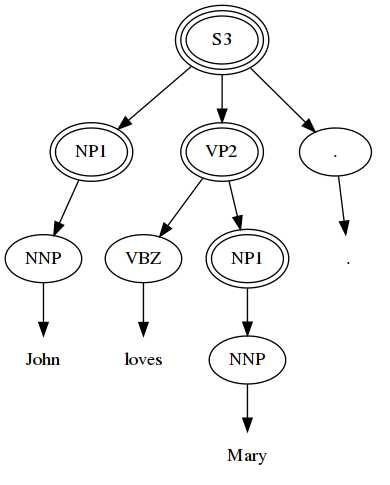
\includegraphics[scale=0.5]{figures/dots/example1.png}
\caption{~\ref{sec:example1}-ben leírt IRTG által generált levezetési fa a \textit{John Loves Mary.} mondat TT-jére.}
\label{fig:example1}
\end{figure}

\begin{figure}[h]
\begin{verbatim}
@(
	S3( *, VP2( VBZ( loves ),  NP1( NNP( Mary ) ) ), .( . ) ), 
	NP1( NNP( John ) ) 
)
\end{verbatim}
\caption{~\ref{sec:example1}-ben leírt IRTG tree interpretációjának kimenete \textit{John Loves Mary.} mondat TT-jére.}
\label{cod:example1output}
\end{figure}



%----------------------------------------------------------------------------
\section{Példa 2}
\label{sec:example2}
%----------------------------------------------------------------------------

\begin{figure}[h]
\begin{verbatim}
\begin{verbatim}
S! -> NP( DT, JJ, NN )
[tree] NP3(?1,?2,?3)

DT -> the_DT
[tree] DT(the)

JJ -> black_JJ
[tree] NN(black)

VB -> cat_VB
[tree] VB(cat)
\end{verbatim}
\caption{Egyszerű három bemenetű IRTG a \textit{the black cat} szószerkezet TT-jének generálására}
\label{cod:example2}
\end{figure}

\begin{figure}[h]
\centering
\graphicspath{./}
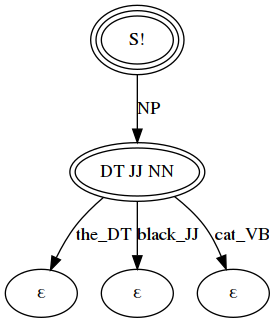
\includegraphics[scale=0.5]{figures/dots/example2.png}
\caption{~\ref{sec:example2}-ben leírt IRTG által generált levezetési fa a \textit{the black cat} szószerkezet TT-jére.}
\label{fig:example2}
\end{figure}

\begin{figure}[h]
\begin{verbatim}
NP3( DT( the ), JJ( black ), NN( cat ) )
\end{verbatim}
\caption{~\ref{sec:example2}-ben leírt IRTG tree interpretációjának kimenete \textit{the black cat} szószerkezet TT-jére. A kimenet maga a  \textit{the black cat} szószerkezet TT-je. }
\label{cod:example2output}
\end{figure}




%----------------------------------------------------------------------------
\section{Példa 3}
\label{sec:example3}
%----------------------------------------------------------------------------

\begin{figure}[h]
\begin{verbatim}
S! -> NP_DT_NP_BAR( DT, NP_BAR)
[tree] @(?2,?1)

NP_BAR -> NP_BAR_JJ_NN(JJ,NN)
[tree] NP3(*,?1,?2)

DT -> the_DT
[tree] DT(the)

JJ -> black_JJ
[tree] NN(black)

VB -> cat_VB
[tree] VB(cat)
\end{verbatim}
\caption{Egyszerű IRTG a \textit{the black cat} szószerkezet TT-jének generálására}
\label{cod:example3}
\end{figure}

\begin{figure}[h]
\centering
\graphicspath{./}
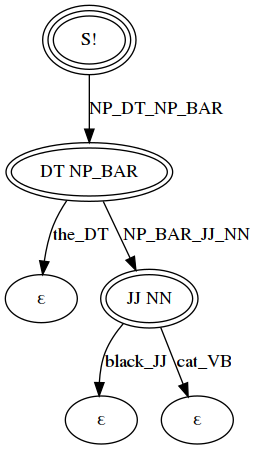
\includegraphics[scale=0.5]{figures/dots/example3.png}
\caption{~\ref{sec:example3}-ban leírt IRTG által generált levezetési fa a \textit{the black cat} szószerkezet TT-jére.}
\label{fig:example3}
\end{figure}

\begin{figure}[h]
\begin{verbatim}
@(  NP3( *, JJ( black ), NN( cat ) ), DT( the ) )
\end{verbatim}
\caption{~\ref{sec:example3}-ben leírt IRTG tree interpretációjának kimenete \textit{the black cat} szószerkezet TT-jére.}
\label{cod:example3output}
\end{figure}




%----------------------------------------------------------------------------
\section{Példa 4}
\label{sec:example4}
%----------------------------------------------------------------------------

\begin{figure}[h]
\begin{verbatim}
S! -> NP_DT_NP_BAR( DT, NP_BAR)
[tree] @(?2,?1)

NP_BAR -> NP_BAR_JJ_NP_BAR(JJ,NP_BAR)
[tree] @(?2,?1)

NP_BAR -> NP_BAR_JJ_NN(JJ,NN)
[tree] NP4(* ,* ,?1 ,?2)

DT -> this_DT
[tree] DT(this)

JJ -> British_JJ
[tree] JJ(British)

JJ -> indastrial_JJ
[tree] JJ(indastrial)

NN -> conglomerate_NN
[tree] NN(conglomerate)
\end{verbatim}
\caption{Egyszerű IRTG a \textit{this British indastrial conglomerate} szószerkezet TT-jének generálására}
\label{cod:example4}
\end{figure}

\begin{figure}[h]
\centering
\graphicspath{./}
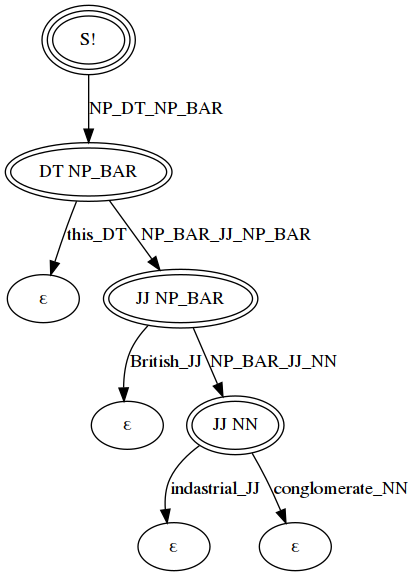
\includegraphics[scale=0.5]{figures/dots/example4.png}
\caption{~\ref{sec:example4}-ben leírt IRTG által generált levezetési fa a \textit{this British indastrial conglomerate} szószerkezet TT-jére.}
\label{fig:example4}
\end{figure}




%----------------------------------------------------------------------------
\section{Példa 5}
\label{sec:example5}
%----------------------------------------------------------------------------

\begin{figure}[h]
\begin{verbatim}
S! -> root_nsubj_NP_S_BAR(NP, S_BAR)
[ud] merge(
			f_dep(merge("(Root/Root :root r<root> :nsubj (d<dep>))", r_dep(?1))),
	 		?2
	 		)

S_BAR -> S_BAR_VP_PUNCT(VP, PUNCT)
[ud] ?1

VP -> dobj_VB_NP(VB,NP)
[ud] merge(f_dep(merge("(r<root> :dobj (d<dep>))", r_dep(?2))),?1)

NP -> NP_NN(NN)
[ud] ?1


NN -> John_NNP
[ud] "(John<root> / John)"

NN -> Mary_NNP
[ud] "(Mary<root> / Mary)"

VB -> loves_VBZ
[ud] "(loves<root> / loves)"

PUNCT -> punct_PUNCT
[ud] "(punct<root> / punct)"
\end{verbatim}
\caption{Egyszerű IRTG a \textit{John Loves Mary.} mondat ud gráfjánek generálására}
\label{cod:example5}
\end{figure}

\begin{figure}[h]
\centering
\graphicspath{./}
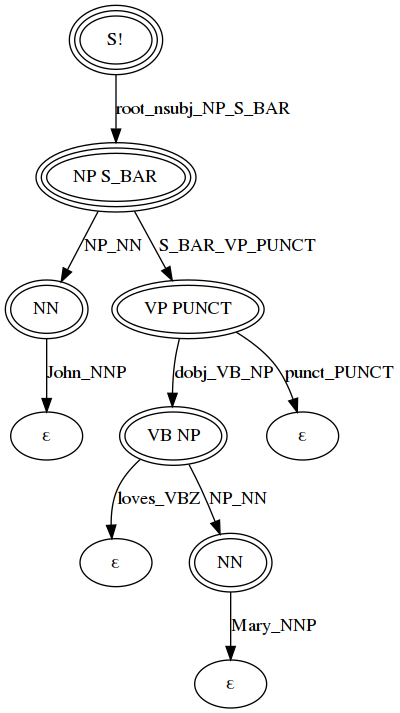
\includegraphics[scale=0.5]{figures/dots/example5_1.png}
\caption{~\ref{sec:example5}-ben leírt IRTG által generált levezetési fa a \textit{John loves Mary.} szószerkezet ud-jét leíró s-graph-ra}
\label{fig:example5.1}
\end{figure}

\begin{figure}[h]
\begin{verbatim}
merge(
	f_dep( merge(
		"(Root/Root :root r<root> :nsubj (d<dep>))",
 		r_dep( "(John<root> / John)" )
		) ),
	 merge(
		f_dep( merge(
					"(r<root> :dobj (d<dep>))", 
					r_dep( "(Mary<root> / Mary)" )
					) ),
 		“(loves<root> / loves)”
		)
	)
\end{verbatim}
\caption{~\ref{sec:example5} ud interpretációjának kimenete}
\label{fig:example5ud}
\end{figure}

\begin{figure}[h]
\centering
\graphicspath{./}
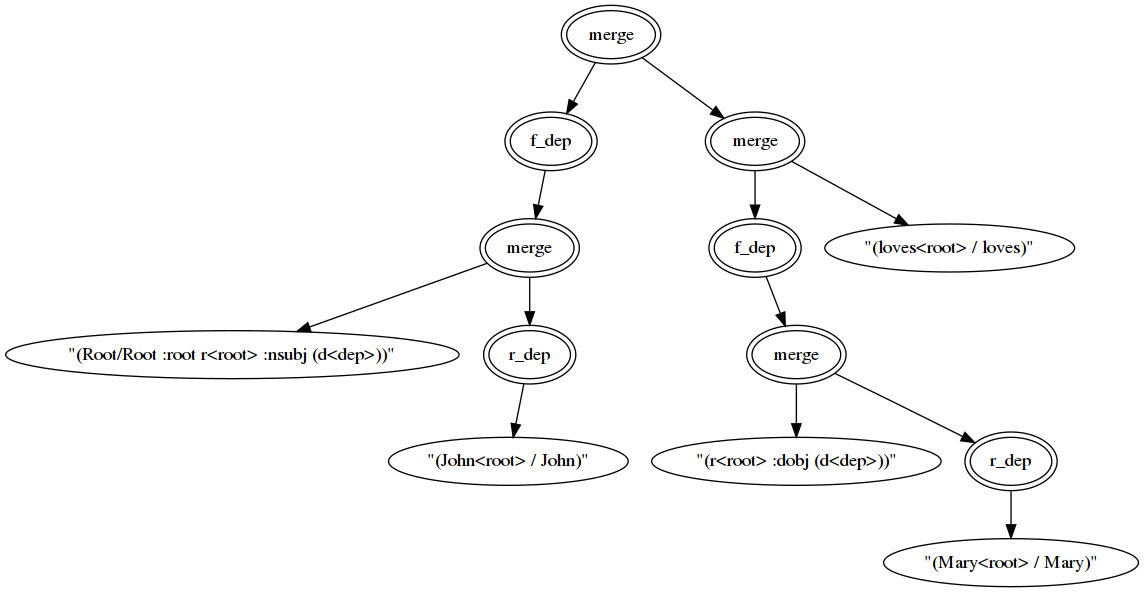
\includegraphics[scale=0.4]{figures/dots/example5_2.png}
\caption{~\ref{sec:example5}-ben leírt IRTG ud interpretációja által generált s-graph kifejezés műveleti fája}
\label{fig:example5.2}
\end{figure}

"(Root/Root :root loves<root>/loves :nsubj (John/John) :dobj (Mary/Mary))"
\begin{figure}[h]
\centering
\graphicspath{./}
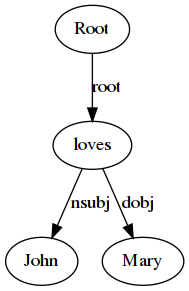
\includegraphics[scale=0.5]{figures/dots/example5_3.png}
\caption{~\ref{sec:example5}-ben leírt IRTG ud interpretációja által generált s-graph kifejezés végeredménye}
\label{fig:example5.3}
\end{figure}




%----------------------------------------------------------------------------
\section{Példa 6}
\label{sec:example6}
%----------------------------------------------------------------------------

\begin{figure}[h]
\begin{verbatim}
S! -> root_nsubj_NP_S_BAR(NP, S_BAR)
[tree] @(?2,?1)
[ud] merge(
			f_dep(merge("(Root/Root :root r<root> :nsubj (d<dep>))", r_dep(?1))),
			?2
			)
[fourlang] merge(
				f_dep(merge("(Root/Root :root r<root> :1,0 (d<dep>))", r_dep(?1))),
				?2
				)

S_BAR -> S_NP_VP(VP, PUNCT)
[tree] S3( *, ?1, ?2)
[ud] ?1
[fourlang] ?1

VP -> dobj_VB_NP(VB,NP)
[tree] VP2(?1,?2)
[ud] merge(
			f_dep(merge("(r<root> :dobj (d<dep>))", r_dep(?2))),
			?1
			)
[fourlang] merge(
				f_dep(merge("(r<root> :2 (d<dep>))", r_dep(?2))),
				?1
				)

NP -> NP_NN(NN)
[tree] NP1(?1)
[ud] ?1
[fourlang] ?1


NN -> John_NNP
[tree] NNP(John)
[ud] "(John<root> / John)"
[fourlang] "(John<root> / John)"

NN -> Mary_NNP
[tree] NNP(Mary)
[ud] "(Mary<root> / Mary)"
[fourlang] "(Mary<root> / Mary)"

VB -> loves_VBZ
[tree] VBZ(loves)
[ud] "(loves<root> / loves)"
[fourlang] "(loves<root> / loves)"

PUNCT -> punct_PUNCT
[tree] .(.)
[ud] "(punct<root> / punct)"
[fourlang] "(punct<root> / punct)"
\end{verbatim}
\caption{IRTG három algebrával a \textit{John Loves Mary.} mondat szintaktikai fájának, ud gráfjának és 4lang gráfjának generálására}
\label{cod:example6}
\end{figure}

\begin{figure}[h]
\centering
\graphicspath{./}
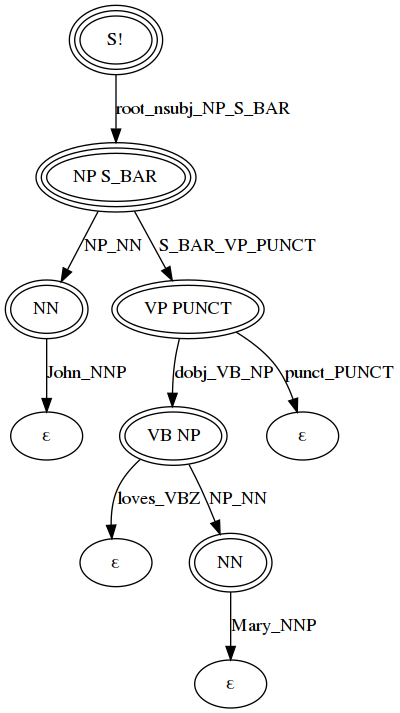
\includegraphics[scale=0.5]{figures/dots/example6_1.png}
\caption{~\ref{sec:example6}-ban leírt IRTG által generált levezetési fa a \textit{John loves Mary.} szószerkezet 4lang-ját leíró s-graph-ra}
\label{fig:example6}
\end{figure}

\begin{figure}[h]
\begin{verbatim}
merge(
	f_dep( 
		merge(
			"(Root/Root :root r<root> :1,0 (d<dep>))",
 			r_dep( 
				"(John<root> / John)" 
				)
			) 
		),
 		merge(
			f_dep( 
					merge(
						"(r<root> :2 (d<dep>))", 
						r_dep( 
							"(Mary<root> / Mary)" 	
							)
						) 
				),
			 “(loves<root> / loves)”
			)
)
\end{verbatim}
\caption{~\ref{sec:example6} fourlang interpretációjának kimenete}
\label{fig:example6fourlang}
\end{figure}

\begin{figure}[h]
\centering
\graphicspath{./}
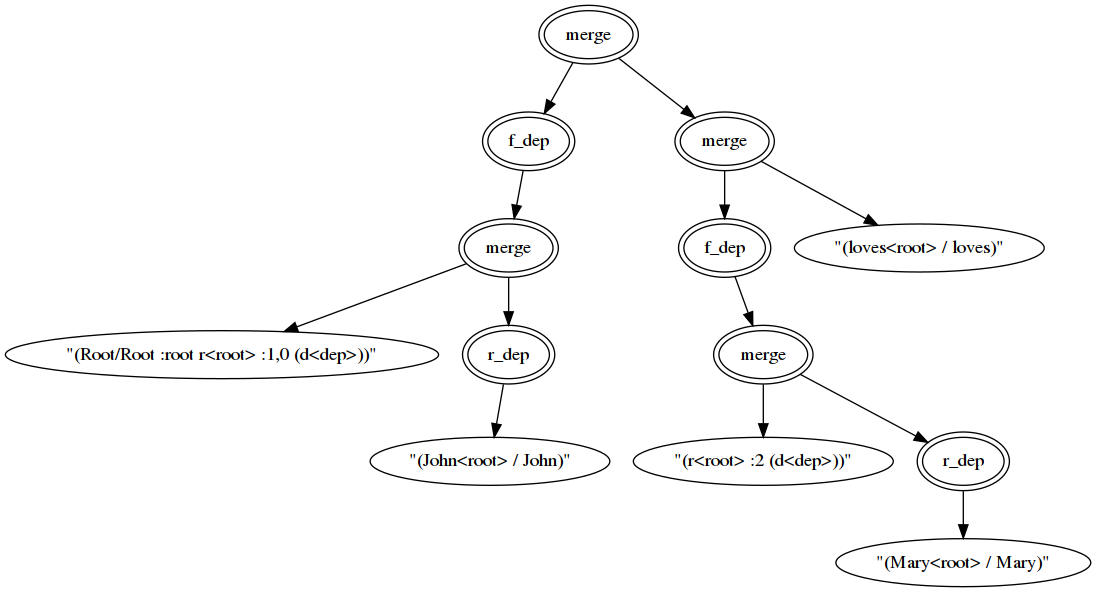
\includegraphics[scale=0.4]{figures/dots/example6_2.png}
\caption{~\ref{sec:example6}-ben leírt IRTG fourlang interpretációja által generált s-graph kifejezés műveleti fája}
\label{fig:example6.2}
\end{figure}

\begin{figure}[h]
\centering
\graphicspath{./}
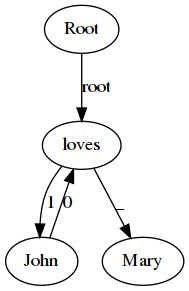
\includegraphics[scale=0.5]{figures/dots/example6_3.png}
\caption{~\ref{sec:example6}-ben leírt IRTG fourlang interpretációja által generált s-graph kifejezés végeredménye}
\label{fig:example6.3}
\end{figure}




%----------------------------------------------------------------------------
\section{Példa 7}
\label{sec:example7}
%----------------------------------------------------------------------------

\begin{figure}[h]
\begin{verbatim}
//merge start
@(																				
	//merge start
	@(																			
		//graph1
		"( [ Root | | Root ] <root- ( [ r | root ] <nsubj- [ d | dep ] ) )",	
		//graph2
	 	"( [ John | root | John ] )",
	 	//tag of graph1
		dep,							
		//tag of graph2
		root,						
		//tag to forget	
		dep							
	//merge end
	),								
	//merge start
 	@(								
 		//merge start
		@(							
			//graph1
			"([ r | root ] <dobj- [ d | dep ] )", 		
			//graph2	
			"( [ Mary | root | Mary] )",
			//tag of graph1				
			dep,						
			//tag of graph2
			root,					
			//tag to forget	
			dep						
		//merge end
		) ,							
		//graph2
		“( [ loves | root | loves ] )”
	//megre end					
	)								
//merge end
)									
\end{verbatim}
\caption{Példa kód az SGA fejlesztésével kapcsolatos koncepció szemléltetésére.
			A példa a \textit{John loves Mary.} mondat UD-gráfjára adott kimenetet dolgozza fel az új szintaxissal.}
\label{cod:example7}
\end{figure}



%----------------------------------------------------------------------------
\section{Példa 8}
\label{sec:example8}
%----------------------------------------------------------------------------

\begin{verbatim}


//merge the root of the left graph with root of the right graph
( 
//merge the dep of left graph with the root of the right graph, then we forget dep
( "( [ Root | | Root ] <root- ( [ r | root ] <nsubj- [ d | dep ] ) )" 
>dep@root< 
"( [ John | root | John ] )" X dep ) 

>root@root<

//merge the root of the left graph with root of the right graph
( 

//merge the dep of left graph with the root of the right graph, then we forget dep
( "([ r | root ] <dobj- [ d | dep ] )" 
>dep@root< 	//merge on dep of left graph and root of right graph
"( [ Mary | root | Mary ]  )" X	dep ) 

>root@root<	//merge on root of left graph and root of right graph

“( [ loves | root | loves ]  )” )

)
\end{verbatim}



%----------------------------------------------------------------------------
\section{Példa IRTG1}
\label{sec:exampleIRTG1}
%----------------------------------------------------------------------------
\begin{verbatim}
{= 
irtgBase : Temp := 
	{|
		{@e@}{@t@}{$left$} -> {$header$}
		{@e@}{@t@}[string] {$string$}
		{@e@}{@t@}[tree] {$syntax_tree$}
		{@e@}{@t@}[ud] {$ud_graph$}
		{@e@}{@t@}[4lang] {$fourlang_graph$}
	|}
=}
{= 
irtgDataBase : Type  :=  left, header, string, syntax_tree, ud_graph, fourlang_graph : Temp
=}
{= 
irtgData : irtgDataBase  :=  
		left		:={|{$word_class$}|},
		header		:={|{$word$}_{$word_class$}|},
		string		:={|{$word$}|},
		syntax_tree	:={|{$word_class$}({$word$})|},
		ud_graph	:={|"({$word$}<root>\{$word$})"|},
		fourlang_graph	:={|"({$concept$}<root>\{$concept$})"|}
=}
{= 
termBase : Temp  :=  {+ irtgBase :+ irtgData +}
=}
{= 
termDataBase : Type  :=  word_class, word, concept : Template
=}
{=data0 :termDataBase  := word_class := {"NN"}, word := {"dog"}, concept := {"dog"} =}
{=data1 :termDataBase  := word_class := {"NN"}, word := {"cat"}, concept := {"cat"} =}
{=data2 :termDataBase  := word_class := {"NN"}, word := {"fish"}, concept := {"fish"} =}
{=data3 :termDataBase  := word_class := {"NN"}, word := {"mouse"}, concept := {"mouse"} =}
{=data4 :termDataBase  := word_class := {"NN"}, word := {"lion"}, concept := {"lion"} =}
{=data5 :termDataBase  := word_class := {"NN"}, word := {"monkey"}, concept := {"monkey"} =}
{=data6 :termDataBase  := word_class := {"NN"}, word := {"fox"}, concept := {"fox"} =}
{=data7 :termDataBase  := word_class := {"NN"}, word := {"bird"}, concept := {"bird"} =}
{=data8 :termDataBase  := word_class := {"NN"}, word := {"tiger"}, concept := {"tiger"} =}
{=data9 :termDataBase  := word_class := {"NN"}, word := {"owl"}, concept := {"owl"} =}
{* 
	{+ 
	termBase.copy :+ data0 : 
		left.cont.word_class 		:+ word_class,
		header.cont.word 		:+ word,
		header.cont.word_class 		:+ word_class,
		string.cont.word	 	:+ word,
		syntax_tree.cont.word_class	:+ word_class,
		syntax_tree.cont.word 		:+ word,
		ud_graph.cont.word.0		:+ word,
		ud_graph.cont.word.1		:+ word,
		fourlang_graph.cont.concept.0	:+ concept,
		fourlang_graph.cont.concept.1	:+ concept
	+}
*}
{@e@}
{* 
	{+ 
	termBase.copy :+ data1 : 
		left.cont.word_class 		:+ word_class,
		header.cont.word 		:+ word,
		header.cont.word_class 		:+ word_class,
		string.cont.word	 	:+ word,
		syntax_tree.cont.word_class	:+ word_class,
		syntax_tree.cont.word 		:+ word,
		ud_graph.cont.word.0		:+ word,
		ud_graph.cont.word.1		:+ word,
		fourlang_graph.cont.concept.0	:+ concept,
		fourlang_graph.cont.concept.1	:+ concept
	+}
*}
{@e@}
{* 
	{+ 
	termBase.copy :+ data2 : 
		left.cont.word_class 		:+ word_class,
		header.cont.word 		:+ word,
		header.cont.word_class 		:+ word_class,
		string.cont.word	 	:+ word,
		syntax_tree.cont.word_class	:+ word_class,
		syntax_tree.cont.word 		:+ word,
		ud_graph.cont.word.0		:+ word,
		ud_graph.cont.word.1		:+ word,
		fourlang_graph.cont.concept.0	:+ concept,
		fourlang_graph.cont.concept.1	:+ concept
	+}
*}
{@e@}
{* 
	{+ 
	termBase.copy :+ data3 : 
		left.cont.word_class 		:+ word_class,
		header.cont.word 		:+ word,
		header.cont.word_class 		:+ word_class,
		string.cont.word	 	:+ word,
		syntax_tree.cont.word_class	:+ word_class,
		syntax_tree.cont.word 		:+ word,
		ud_graph.cont.word.0		:+ word,
		ud_graph.cont.word.1		:+ word,
		fourlang_graph.cont.concept.0	:+ concept,
		fourlang_graph.cont.concept.1	:+ concept
	+}
*}
{@e@}
{* 
	{+ 
	termBase.copy :+ data4 : 
		left.cont.word_class 		:+ word_class,
		header.cont.word 		:+ word,
		header.cont.word_class 		:+ word_class,
		string.cont.word	 	:+ word,
		syntax_tree.cont.word_class	:+ word_class,
		syntax_tree.cont.word 		:+ word,
		ud_graph.cont.word.0		:+ word,
		ud_graph.cont.word.1		:+ word,
		fourlang_graph.cont.concept.0	:+ concept,
		fourlang_graph.cont.concept.1	:+ concept
	+}
*}
{@e@}
{* 
	{+ 
	termBase.copy :+ data5 : 
		left.cont.word_class 		:+ word_class,
		header.cont.word 		:+ word,
		header.cont.word_class 		:+ word_class,
		string.cont.word	 	:+ word,
		syntax_tree.cont.word_class	:+ word_class,
		syntax_tree.cont.word 		:+ word,
		ud_graph.cont.word.0		:+ word,
		ud_graph.cont.word.1		:+ word,
		fourlang_graph.cont.concept.0	:+ concept,
		fourlang_graph.cont.concept.1	:+ concept
	+}
*}
{@e@}
{* 
	{+ 
	termBase.copy :+ data6 : 
		left.cont.word_class 		:+ word_class,
		header.cont.word 		:+ word,
		header.cont.word_class 		:+ word_class,
		string.cont.word	 	:+ word,
		syntax_tree.cont.word_class	:+ word_class,
		syntax_tree.cont.word 		:+ word,
		ud_graph.cont.word.0		:+ word,
		ud_graph.cont.word.1		:+ word,
		fourlang_graph.cont.concept.0	:+ concept,
		fourlang_graph.cont.concept.1	:+ concept
	+}
*}
{@e@}
{* 
	{+ 
	termBase.copy :+ data7 : 
		left.cont.word_class 		:+ word_class,
		header.cont.word 		:+ word,
		header.cont.word_class 		:+ word_class,
		string.cont.word	 	:+ word,
		syntax_tree.cont.word_class	:+ word_class,
		syntax_tree.cont.word 		:+ word,
		ud_graph.cont.word.0		:+ word,
		ud_graph.cont.word.1		:+ word,
		fourlang_graph.cont.concept.0	:+ concept,
		fourlang_graph.cont.concept.1	:+ concept
	+}
*}
{@e@}
{* 
	{+ 
	termBase.copy :+ data8 : 
		left.cont.word_class 		:+ word_class,
		header.cont.word 		:+ word,
		header.cont.word_class 		:+ word_class,
		string.cont.word	 	:+ word,
		syntax_tree.cont.word_class	:+ word_class,
		syntax_tree.cont.word 		:+ word,
		ud_graph.cont.word.0		:+ word,
		ud_graph.cont.word.1		:+ word,
		fourlang_graph.cont.concept.0	:+ concept,
		fourlang_graph.cont.concept.1	:+ concept
	+}
*}
{@e@}
{* 
	{+ 
	termBase.copy :+ data9 : 
		left.cont.word_class 		:+ word_class,
		header.cont.word 		:+ word,
		header.cont.word_class 		:+ word_class,
		string.cont.word	 	:+ word,
		syntax_tree.cont.word_class	:+ word_class,
		syntax_tree.cont.word 		:+ word,
		ud_graph.cont.word.0		:+ word,
		ud_graph.cont.word.1		:+ word,
		fourlang_graph.cont.concept.0	:+ concept,
		fourlang_graph.cont.concept.1	:+ concept
	+}
*}
{@e@}
\end{verbatim}


%----------------------------------------------------------------------------
\section{Példa IRTG2}
\label{sec:exampleIRTG2}
%----------------------------------------------------------------------------
\begin{verbatim}
{= 
dataFile :File := {"/home/boss/Documents/Git/SlimeAnUTLE/test_codes/irtg_example2data"};
result :List:Temp := {+ dataFile.termBase :+ dataFile.datas +} 
=}
{*
{+ 
result :+ dataFile.datas : 
	0.slots.iter:+0, 
	1.slots.iter:+1, 
	2.slots.iter:+2, 
	3.slots.iter:+3, 
	4.slots.iter:+4, 
	5.slots.iter:+5, 
	6.slots.iter:+6, 
	7.slots.iter:+7, 
	8.slots.iter:+8, 
	9.slots.iter:+9 
+}: {@e@} 
*}

\end{verbatim}

\begin{verbatim}
{# Data for example 2 #}
{= 
irtgBase : Temp := 
	{|
		{@e;t@}{$left$} -> {$header$}
		{@e;t@}[string] {$string$}
		{@e;t@}[tree] {$syntax_tree$}
		{@e;t@}[ud] {$ud_graph$}
		{@e;t@}[4lang] {$fourlang_graph$}
	|};

irtgDataBase : Type  :=  left, header, string, syntax_tree, ud_graph, fourlang_graph : Temp;

irtgData : irtgDataBase  :=  
	{|
		{$word_class$};{$word$}_{$word_class$};
		{$word$};
		{$word_class$}({$word$});
		"({$word$}<root>\{$word$})";
		"({$concept$}<root>\{$concept$})"
	|};

termBase : Temp  :=  {+ irtgBase :+ irtgData +};

termDataBase : Type  :=  word_class, word, concept : Template;

datas :List:termDataBase :=
	{= :termDataBase  := 	{"NN"}, {"dog"},   {"dog"} 	=},
	{= :termDataBase  := 	{"NN"}, {"cat"},   {"cat"} 	=},
	{= :termDataBase  := 	{"NN"}, {"fish"},  {"fish"} 	=},
	{= :termDataBase  := 	{"NN"}, {"mouse"}, {"mouse"} 	=},
	{= :termDataBase  :=	{"NN"}, {"lion"},  {"lion"} 	=},
	{= :termDataBase  := 	{"NN"}, {"monkey"},{"monkey"} 	=},
	{= :termDataBase  := 	{"NN"}, {"fox"},   {"fox"} 	=},
	{= :termDataBase  := 	{"NN"}, {"bird"},  {"bird"} 	=},
	{= :termDataBase  := 	{"NN"}, {"tiger"}, {"tiger"} 	=},
	{= :termDataBase  := 	{"NN"}, {"owl"},   {"owl"} 	=}
=}

\end{verbatim}

%----------------------------------------------------------------------------
\section{Példa IRTG3}
\label{sec:exampleIRTG3}
%----------------------------------------------------------------------------
\begin{verbatim}
{= 
irtgBase,IB : Temp := 
	{|
		<@e;t <$left  -> [$header
		<@e;t [string] [$string
		<@e;t [tree] [$syntax_tree
		<@e;t [ud] [$ud_graph
		<@e;t [4lang] [$fourlang_graph
	|}

IDB,irtgDataBase : Type  :=  left, header, string, syntax_tree, ud_graph, fourlang_graph : Template

irtgData,ID : IDB  :=  
	{|
		<$word_class ;<$word _<$word_class ;
		<$word ;
		<$word_class (<$word );
		"(<$word <root>\<$word )";
		"(<$concept <root>\<$concept )"
	|}

termBase,TB : Temp  :=  <+IB:+ID

TDB,termDataBase : Type  :=  word_class, word, concept : Temp

datas,D :List:TDB :=
	 [=:TDB:= [|NN;dog;dog 
	,[=:TDB:= [|NN;cat;cat 
	,[=:TDB:= [|NN;owl;owl 
	,[=:TDB:= [|NN;fox;fox 
	,[=:TDB:= [|NN;fish;fish 
	,[=:TDB:= [|NN;lion;lion 
	,[=:TDB:= [|NN;bird;bird 
	,[=:TDB:= [|NN;mouse;mouse 
	,[=:TDB:= [|NN;tiger;tiger 
	,[=:TDB:= [|NN;monkey;monkey 

result,R :List:Temp := <+TB:+D 
=}
<*{+ 
R :+ D : 
	0.slots.iter:+0, 
	1.slots.iter:+1, 
	2.slots.iter:+2, 
	3.slots.iter:+3, 
	4.slots.iter:+4, 
	5.slots.iter:+5, 
	6.slots.iter:+6, 
	7.slots.iter:+7, 
	8.slots.iter:+8, 
	9.slots.iter:+9 
+}:<@e

\end{verbatim}


%----------------------------------------------------------------------------
\section{Példa IRTG4}
\label{sec:exampleIRTG4}
%----------------------------------------------------------------------------
\begin{verbatim}
{= 
irtgBase,IB : Temp := 
	{|
		<@e;t //[$comm
		<@e;t <$left  -> [$header
		<@e;t [string] [$string
		<@e;t [tree] [$tree
		<@e;t [ud] [$ud
		<@e;t [4lang] [$four
	|}

IDB,irtgDataBase : Type  :=  comm, left, header, string, tree, ud, four : Temp

irtgData1,ID1 : IDB  :=  
	{|
		{$comm$};
		NP;_NP2_{$edge_ud$}_{$arg1$}_{$arg2$}({$arg1$}, {$arg2$}); 
        	*(?1, ?2);
		NP2(?1,?2); 
		merge(f_dep(merge("(r<root> :{$edge_ud$} (d<dep>))",r_dep(?1))),?2);
		merge(f_dep(merge("(r<root> :{$edge_4lang$}) (d<dep>))",r_dep(?1))),?2)
	|}

irtgData2,ID2 : IDB  := ID1.0, ID1.1, ID1.2, ID1.3, ID1.4, ID1.5,
	{|?2|}
	

irtgData3,ID3 : IDB  := ID1.0, ID1.1, ID1.2, ID1.3, ID1.4, ID1.5,
	{|f_dep(merge(merge(?1, "(HAS / HAS :1 (d<dep>) :2 (r<root>))"), r_dep(?2)))|}

nounPhraseBase1,NPB1 : Temp  :=  <+IB.copy:+ID1
nounPhraseBase1,NPB2 : Temp  :=  <+IB.copy:+ID2
nounPhraseBase1,NPB3 : Temp  :=  <+IB.copy:+ID3

NPDB,nounPhraseDataBase : Type  :=  comm,  arg1, arg2, edge_ud, edge_4lang : Text

datas1,D1 :List:NPDB :=
	 [=:NPDB:= {"cute cat"}			,{"JJ"}	,{"NN"}		,{"amod"}	,{"0"}
	,[=:NPDB:= {"electricity charges"}	,{"NN"}	,{"NNS"}	,{"compound"}	,{"0_compound_nouns"}
	,[=:NPDB:= {"car safety"}		,{"NN"}	,{"NN"}		,{"compound"}	,{"0_compound_nouns"}
	,[=:NPDB:= {"one dog"}			,{"CD"}	,{"NN"}		,{"nummod"}	,{"0"}
	,[=:NPDB:= {"three dogs"}		,{"CD"}	,{"NNS"}	,{"nummod"}	,{"0"}
	,[=:NPDB:= {"cute cats"}		,{"JJ"}	,{"NNS"}	,{"amod"}	,{"0"}
	,[=:NPDB:= {"John Smith"}		,{"NNP"},{"NNP"}	,{"flat"}	,{"0_flat_name"}
	
datas2,D2 :List:NPDB :=
	 [=:NPDB:= {"the Examiner"}	,{"DT"}	,{"NNP"}	,{"det"}
	,[=:NPDB:= {"a cat"}		,{"DT"}	,{"NN"}		,{"det"}
	,[=:NPDB:= {"the cats"}		,{"DT"}	,{"NNS"}	,{"det"}
	
datas3,D3 :List:NPDB :=
	 [=:NPDB:= {"my cat"}		,{"PRPDOLLAR"}	,{"NN"}		,{"nmod:poss"}
	,[=:NPDB:= {"my cats"}		,{"PRPDOLLAR"}	,{"NNS"}	,{"nmod:poss"}

result1,R1 :List:Temp := <+NPB1:+D1
result2,R2 :List:Temp := <+NPB2:+D2
result3,R3 :List:Temp := <+NPB3:+D3
=}
<*{+ 
R1 :+ D1 : 
	0.slots.iter:+0, 
	1.slots.iter:+1, 
	2.slots.iter:+2, 
	3.slots.iter:+3, 
	4.slots.iter:+4, 
	5.slots.iter:+5, 
	6.slots.iter:+6
R2 :+ D2 : 
	0.slots.iter:+0, 
	1.slots.iter:+1, 
	2.slots.iter:+2
R3 :+ D3 : 
	0.slots.iter:+0, 
	1.slots.iter:+1
+}:<@e 

\end{verbatim}


%----------------------------------------------------------------------------
\section{Példa ANTLR}
\label{sec:exampleANTLR}
%----------------------------------------------------------------------------

\begin{verbatim}
{=
shortRuleBase, SRB	:Temp := {|<$typeB _<$typeM  : '<$pattB;pattM ' -> 
					pushMode(<$modeB _<$modeM )<@sc <$wrap |}
longRuleBase, LRB    	:Temp := {|<$typeB _<$typeM _<$fromB _<$fromM  : '<$pattB;pattM ' ->
					type(<$typeB _<$typeM ), pushMode(<$modeB _<$modeM )<@sc <$wrap |}

BDB,bracDataBase : Type := typeB, pattB, modeB :Temp
bracDatas,BD :List:BDB :=
	 [=:BDB:= [|BOB;{;B
	,[=:BDB:= [|OLB;[;O
	,[=:BDB:= [|COB;<;C

MDB,modeDataBase : Type := typeM, pattM, modeM, wrap :Temp
modeDatas3,MD3 :List:MDB :=
	 [=:MDB:= [|SLOT;$;SLSP;<@e 
	,[=:MDB:= [|SPEC;@;SLSP;<@e 
	,[=:MDB:= [|TEXT;";TEXT;<@e;e 
modeDatas9,MD9 :List:MDB := MD3.0, MD3.1
	,[=:MDB:= [|REFE;&;REFE;<@e 
	,[=:MDB:= [|EXTE;*;OPER;<@e 
	,[=:MDB:= [|PLUS;+;OPER;<@e 
	,[=:MDB:= [|DECL;=;OPER;<@e 
	,[=:MDB:= [|DELE;X;OPER;<@e 
	,[=:MDB:= [|TEXT;";TEXT;<@e 
	,[=:MDB:= [|TEMP;|;TEMP;<@e;e 
fromBData ,FBD	:List:Temp := [|B;O;C
fromMData ,FMD	:List:Temp := [|O;T
=}

{=
datasBasic, DB	: List:Temp := [+SRB:+BD

dataBasicBloc, DBB	:List:Temp := [+ DB.0 :+ MD9
dataBasicOnel, DBO	:List:Temp := [+ DB.1 :+ MD9
dataBasicComp, DBC	:List:Temp := [+ DB.2 :+ MD9
=}
{*
{&List:Temp:&DB[BOC]&}
{@e@}
*}

{=
datasLong, DL		: List:Temp := [+ LRB.fromM :+ FMD
DLOper, DLO	: List:Temp := [+ DL.0.fromB :+ FBD
DLTemp, DLT	: List:Temp := [+ DL.1.fromB :+ FBD

DLBlocOper, DLBO: List:Temp := [+ DLO.0 :+ BD
DLOnelOper, DLOO: List:Temp := [+ DLO.1 :+ BD
DLCompOper, DLCO: List:Temp := [+ DLO.2 :+ BD
DLBlocTemp, DLBT: List:Temp := [+ DLT.0 :+ BD
DLOnelTemp, DLOT: List:Temp := [+ DLT.1 :+ BD
DLCompTemp, DLCT: List:Temp := [+ DLT.2 :+ BD
 
DLBOBloc, DLBOB: List:Temp := [+ DLBO.0 :+ MD9
DLBOOnel, DLBOO: List:Temp := [+ DLBO.1 :+ MD9
DLBOComp, DLBOC: List:Temp := [+ DLBO.2 :+ MD9
DLOOBloc, DLOOB: List:Temp := [+ DLOO.0 :+ MD9
DLOOOnel, DLOOO: List:Temp := [+ DLOO.1 :+ MD9
DLOOComp, DLOOC: List:Temp := [+ DLOO.2 :+ MD9
DLCOBloc, DLCOB: List:Temp := [+ DLCO.0 :+ MD9
DLCOOnel, DLCOO: List:Temp := [+ DLCO.1 :+ MD9
DLCOComp, DLCOC: List:Temp := [+ DLCO.2 :+ MD9
DLBTBloc, DLBTB: List:Temp := [+ DLBT.0 :+ MD3
DLBTOnel, DLBTO: List:Temp := [+ DLBT.1 :+ MD3
DLBTComp, DLBTC: List:Temp := [+ DLBT.2 :+ MD3
DLOTBloc, DLOTB: List:Temp := [+ DLOT.0 :+ MD3
DLOTOnel, DLOTO: List:Temp := [+ DLOT.1 :+ MD3
DLOTComp, DLOTC: List:Temp := [+ DLOT.2 :+ MD3
DLCTBloc, DLCTB: List:Temp := [+ DLCT.0 :+ MD3
DLCTOnel, DLCTO: List:Temp := [+ DLCT.1 :+ MD3
DLCTComp, DLCTC: List:Temp := [+ DLCT.2 :+ MD3
=}

{*
	{&List:Temp:&DLBO[BOC]&}{@e@}
	{&List:Temp:&DLOO[BOC]&}{@e@}
	{&List:Temp:&DLCO[BOC]&}{@e@}
	{@e@}
	{&List:Temp:&DLBT[BOC]&}{@e@}
	{&List:Temp:&DLOT[BOC]&}{@e@}
	{&List:Temp:&DLCT[BOC]&}{@e@}
*}


\end{verbatim}

Ilyen kimenetet ad:

\begin{verbatim}
BOB_SLOT : '{$' -> pushMode(B_SLSP);
BOB_SPEC : '{@' -> pushMode(B_SLSP);
BOB_REFE : '{&' -> pushMode(B_REFE);
BOB_EXTE : '{*' -> pushMode(B_OPER);
BOB_PLUS : '{+' -> pushMode(B_OPER);
BOB_DECL : '{=' -> pushMode(B_OPER);
BOB_DELE : '{X' -> pushMode(B_OPER);
BOB_TEXT : '{"' -> pushMode(B_TEXT);
BOB_TEMP : '{|' -> pushMode(B_TEMP);

OLB_SLOT : '[$' -> pushMode(O_SLSP);
OLB_SPEC : '[@' -> pushMode(O_SLSP);
OLB_REFE : '[&' -> pushMode(O_REFE);
OLB_EXTE : '[*' -> pushMode(O_OPER);
OLB_PLUS : '[+' -> pushMode(O_OPER);
OLB_DECL : '[=' -> pushMode(O_OPER);
OLB_DELE : '[X' -> pushMode(O_OPER);
OLB_TEXT : '["' -> pushMode(O_TEXT);
OLB_TEMP : '[|' -> pushMode(O_TEMP);

COB_SLOT : '<$' -> pushMode(C_SLSP);
COB_SPEC : '<@' -> pushMode(C_SLSP);
COB_REFE : '<&' -> pushMode(C_REFE);
COB_EXTE : '<*' -> pushMode(C_OPER);
COB_PLUS : '<+' -> pushMode(C_OPER);
COB_DECL : '<=' -> pushMode(C_OPER);
COB_DELE : '<X' -> pushMode(C_OPER);
COB_TEXT : '<"' -> pushMode(C_TEXT);
COB_TEMP : '<|' -> pushMode(C_TEMP);


BOB_SLOT_B_O : '{$' -> type(BOB_SLOT), pushMode(B_SLSP);
BOB_SPEC_B_O : '{@' -> type(BOB_SPEC), pushMode(B_SLSP);
BOB_REFE_B_O : '{&' -> type(BOB_REFE), pushMode(B_REFE);
BOB_EXTE_B_O : '{*' -> type(BOB_EXTE), pushMode(B_OPER);
BOB_PLUS_B_O : '{+' -> type(BOB_PLUS), pushMode(B_OPER);
BOB_DECL_B_O : '{=' -> type(BOB_DECL), pushMode(B_OPER);
BOB_DELE_B_O : '{X' -> type(BOB_DELE), pushMode(B_OPER);
BOB_TEXT_B_O : '{"' -> type(BOB_TEXT), pushMode(B_TEXT);
BOB_TEMP_B_O : '{|' -> type(BOB_TEMP), pushMode(B_TEMP);

OLB_SLOT_B_O : '[$' -> type(OLB_SLOT), pushMode(O_SLSP);
OLB_SPEC_B_O : '[@' -> type(OLB_SPEC), pushMode(O_SLSP);
OLB_REFE_B_O : '[&' -> type(OLB_REFE), pushMode(O_REFE);
OLB_EXTE_B_O : '[*' -> type(OLB_EXTE), pushMode(O_OPER);
OLB_PLUS_B_O : '[+' -> type(OLB_PLUS), pushMode(O_OPER);
OLB_DECL_B_O : '[=' -> type(OLB_DECL), pushMode(O_OPER);
OLB_DELE_B_O : '[X' -> type(OLB_DELE), pushMode(O_OPER);
OLB_TEXT_B_O : '["' -> type(OLB_TEXT), pushMode(O_TEXT);
OLB_TEMP_B_O : '[|' -> type(OLB_TEMP), pushMode(O_TEMP);

COB_SLOT_B_O : '<$' -> type(COB_SLOT), pushMode(C_SLSP);
COB_SPEC_B_O : '<@' -> type(COB_SPEC), pushMode(C_SLSP);
COB_REFE_B_O : '<&' -> type(COB_REFE), pushMode(C_REFE);
COB_EXTE_B_O : '<*' -> type(COB_EXTE), pushMode(C_OPER);
COB_PLUS_B_O : '<+' -> type(COB_PLUS), pushMode(C_OPER);
COB_DECL_B_O : '<=' -> type(COB_DECL), pushMode(C_OPER);
COB_DELE_B_O : '<X' -> type(COB_DELE), pushMode(C_OPER);
COB_TEXT_B_O : '<"' -> type(COB_TEXT), pushMode(C_TEXT);
COB_TEMP_B_O : '<|' -> type(COB_TEMP), pushMode(C_TEMP);


BOB_SLOT_O_O : '{$' -> type(BOB_SLOT), pushMode(B_SLSP);
BOB_SPEC_O_O : '{@' -> type(BOB_SPEC), pushMode(B_SLSP);
BOB_REFE_O_O : '{&' -> type(BOB_REFE), pushMode(B_REFE);
BOB_EXTE_O_O : '{*' -> type(BOB_EXTE), pushMode(B_OPER);
BOB_PLUS_O_O : '{+' -> type(BOB_PLUS), pushMode(B_OPER);
BOB_DECL_O_O : '{=' -> type(BOB_DECL), pushMode(B_OPER);
BOB_DELE_O_O : '{X' -> type(BOB_DELE), pushMode(B_OPER);
BOB_TEXT_O_O : '{"' -> type(BOB_TEXT), pushMode(B_TEXT);
BOB_TEMP_O_O : '{|' -> type(BOB_TEMP), pushMode(B_TEMP);

OLB_SLOT_O_O : '[$' -> type(OLB_SLOT), pushMode(O_SLSP);
OLB_SPEC_O_O : '[@' -> type(OLB_SPEC), pushMode(O_SLSP);
OLB_REFE_O_O : '[&' -> type(OLB_REFE), pushMode(O_REFE);
OLB_EXTE_O_O : '[*' -> type(OLB_EXTE), pushMode(O_OPER);
OLB_PLUS_O_O : '[+' -> type(OLB_PLUS), pushMode(O_OPER);
OLB_DECL_O_O : '[=' -> type(OLB_DECL), pushMode(O_OPER);
OLB_DELE_O_O : '[X' -> type(OLB_DELE), pushMode(O_OPER);
OLB_TEXT_O_O : '["' -> type(OLB_TEXT), pushMode(O_TEXT);
OLB_TEMP_O_O : '[|' -> type(OLB_TEMP), pushMode(O_TEMP);

COB_SLOT_O_O : '<$' -> type(COB_SLOT), pushMode(C_SLSP);
COB_SPEC_O_O : '<@' -> type(COB_SPEC), pushMode(C_SLSP);
COB_REFE_O_O : '<&' -> type(COB_REFE), pushMode(C_REFE);
COB_EXTE_O_O : '<*' -> type(COB_EXTE), pushMode(C_OPER);
COB_PLUS_O_O : '<+' -> type(COB_PLUS), pushMode(C_OPER);
COB_DECL_O_O : '<=' -> type(COB_DECL), pushMode(C_OPER);
COB_DELE_O_O : '<X' -> type(COB_DELE), pushMode(C_OPER);
COB_TEXT_O_O : '<"' -> type(COB_TEXT), pushMode(C_TEXT);
COB_TEMP_O_O : '<|' -> type(COB_TEMP), pushMode(C_TEMP);


BOB_SLOT_C_O : '{$' -> type(BOB_SLOT), pushMode(B_SLSP);
BOB_SPEC_C_O : '{@' -> type(BOB_SPEC), pushMode(B_SLSP);
BOB_REFE_C_O : '{&' -> type(BOB_REFE), pushMode(B_REFE);
BOB_EXTE_C_O : '{*' -> type(BOB_EXTE), pushMode(B_OPER);
BOB_PLUS_C_O : '{+' -> type(BOB_PLUS), pushMode(B_OPER);
BOB_DECL_C_O : '{=' -> type(BOB_DECL), pushMode(B_OPER);
BOB_DELE_C_O : '{X' -> type(BOB_DELE), pushMode(B_OPER);
BOB_TEXT_C_O : '{"' -> type(BOB_TEXT), pushMode(B_TEXT);
BOB_TEMP_C_O : '{|' -> type(BOB_TEMP), pushMode(B_TEMP);

OLB_SLOT_C_O : '[$' -> type(OLB_SLOT), pushMode(O_SLSP);
OLB_SPEC_C_O : '[@' -> type(OLB_SPEC), pushMode(O_SLSP);
OLB_REFE_C_O : '[&' -> type(OLB_REFE), pushMode(O_REFE);
OLB_EXTE_C_O : '[*' -> type(OLB_EXTE), pushMode(O_OPER);
OLB_PLUS_C_O : '[+' -> type(OLB_PLUS), pushMode(O_OPER);
OLB_DECL_C_O : '[=' -> type(OLB_DECL), pushMode(O_OPER);
OLB_DELE_C_O : '[X' -> type(OLB_DELE), pushMode(O_OPER);
OLB_TEXT_C_O : '["' -> type(OLB_TEXT), pushMode(O_TEXT);
OLB_TEMP_C_O : '[|' -> type(OLB_TEMP), pushMode(O_TEMP);

COB_SLOT_C_O : '<$' -> type(COB_SLOT), pushMode(C_SLSP);
COB_SPEC_C_O : '<@' -> type(COB_SPEC), pushMode(C_SLSP);
COB_REFE_C_O : '<&' -> type(COB_REFE), pushMode(C_REFE);
COB_EXTE_C_O : '<*' -> type(COB_EXTE), pushMode(C_OPER);
COB_PLUS_C_O : '<+' -> type(COB_PLUS), pushMode(C_OPER);
COB_DECL_C_O : '<=' -> type(COB_DECL), pushMode(C_OPER);
COB_DELE_C_O : '<X' -> type(COB_DELE), pushMode(C_OPER);
COB_TEXT_C_O : '<"' -> type(COB_TEXT), pushMode(C_TEXT);
COB_TEMP_C_O : '<|' -> type(COB_TEMP), pushMode(C_TEMP);



BOB_SLOT_B_T : '{$' -> type(BOB_SLOT), pushMode(B_SLSP);
BOB_SPEC_B_T : '{@' -> type(BOB_SPEC), pushMode(B_SLSP);
BOB_TEXT_B_T : '{"' -> type(BOB_TEXT), pushMode(B_TEXT);

OLB_SLOT_B_T : '[$' -> type(OLB_SLOT), pushMode(O_SLSP);
OLB_SPEC_B_T : '[@' -> type(OLB_SPEC), pushMode(O_SLSP);
OLB_TEXT_B_T : '["' -> type(OLB_TEXT), pushMode(O_TEXT);

COB_SLOT_B_T : '<$' -> type(COB_SLOT), pushMode(C_SLSP);
COB_SPEC_B_T : '<@' -> type(COB_SPEC), pushMode(C_SLSP);
COB_TEXT_B_T : '<"' -> type(COB_TEXT), pushMode(C_TEXT);


BOB_SLOT_O_T : '{$' -> type(BOB_SLOT), pushMode(B_SLSP);
BOB_SPEC_O_T : '{@' -> type(BOB_SPEC), pushMode(B_SLSP);
BOB_TEXT_O_T : '{"' -> type(BOB_TEXT), pushMode(B_TEXT);

OLB_SLOT_O_T : '[$' -> type(OLB_SLOT), pushMode(O_SLSP);
OLB_SPEC_O_T : '[@' -> type(OLB_SPEC), pushMode(O_SLSP);
OLB_TEXT_O_T : '["' -> type(OLB_TEXT), pushMode(O_TEXT);

COB_SLOT_O_T : '<$' -> type(COB_SLOT), pushMode(C_SLSP);
COB_SPEC_O_T : '<@' -> type(COB_SPEC), pushMode(C_SLSP);
COB_TEXT_O_T : '<"' -> type(COB_TEXT), pushMode(C_TEXT);


BOB_SLOT_C_T : '{$' -> type(BOB_SLOT), pushMode(B_SLSP);
BOB_SPEC_C_T : '{@' -> type(BOB_SPEC), pushMode(B_SLSP);
BOB_TEXT_C_T : '{"' -> type(BOB_TEXT), pushMode(B_TEXT);

OLB_SLOT_C_T : '[$' -> type(OLB_SLOT), pushMode(O_SLSP);
OLB_SPEC_C_T : '[@' -> type(OLB_SPEC), pushMode(O_SLSP);
OLB_TEXT_C_T : '["' -> type(OLB_TEXT), pushMode(O_TEXT);

COB_SLOT_C_T : '<$' -> type(COB_SLOT), pushMode(C_SLSP);
COB_SPEC_C_T : '<@' -> type(COB_SPEC), pushMode(C_SLSP);
COB_TEXT_C_T : '<"' -> type(COB_TEXT), pushMode(C_TEXT);

\end{verbatim}

Tehát a sorokat tekintve a felére esett össze a szöveg.
Így is könnyen megfigyelhető a redundancia Slime kódban.
Ha az iterátoros hozzáadások fejlettebbek lesznek, akkor a még nagyjából kétharmad ennyi sorból meglehetett volna oldani.
Jelenleg az iterátoros hozzáadások legkorlátozóbb tényezője a visszatérési érték.
Ennél tömörebb eredményt a nyelv jelen fejlődési fázisában csak a Slime kód template-elésével érhettünk volna el.